\documentclass[tikz,border=5pt]{standalone}
\usepackage[T1]{fontenc}
\usepackage{lmodern}
\usetikzlibrary{arrows.meta,positioning}
\begin{document}
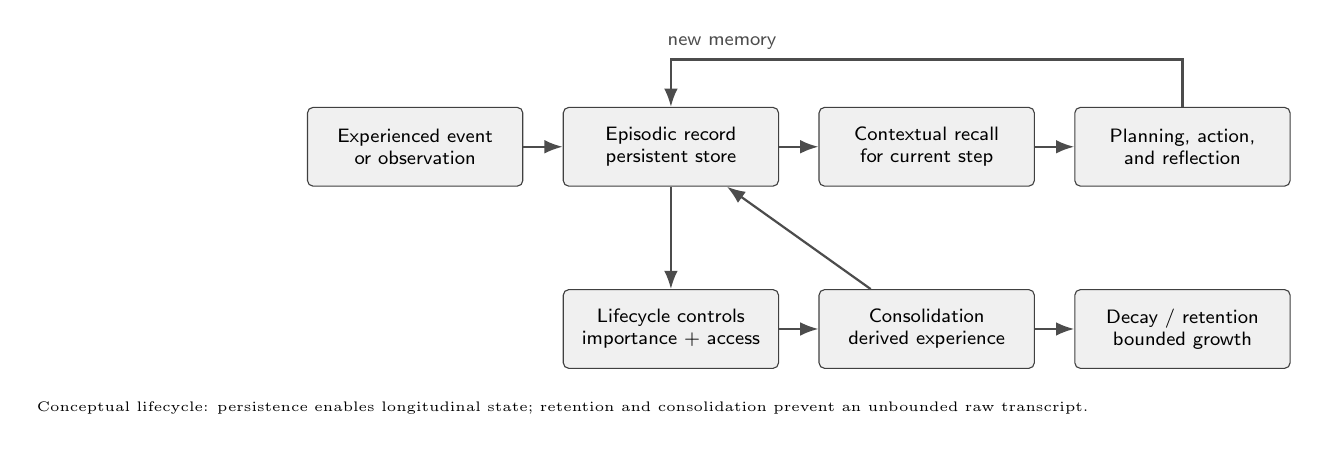
\begin{tikzpicture}[font=\sffamily\scriptsize,>=Latex,
 box/.style={draw=black!75,rounded corners=2pt,fill=black!6,text width=25mm,minimum height=10mm,align=center},
 flow/.style={->,thick,black!70}]
\node[box] (event) {Experienced event\\or observation};
\node[box,right=5mm of event] (episodic) {Episodic record\\persistent store};
\node[box,right=5mm of episodic] (recall) {Contextual recall\\for current step};
\node[box,right=5mm of recall] (action) {Planning, action,\\and reflection};
\draw[flow] (event) -- (episodic);
\draw[flow] (episodic) -- (recall);
\draw[flow] (recall) -- (action);
\draw[flow] (action.north) -- ++(0,6mm) -| node[pos=.45,above]{new memory} (episodic.north);

\node[box,below=13mm of episodic] (lifecycle) {Lifecycle controls\\importance + access};
\node[box,below=13mm of recall] (consolidate) {Consolidation\\derived experience};
\node[box,below=13mm of action] (decay) {Decay / retention\\bounded growth};
\draw[flow] (episodic) -- (lifecycle);
\draw[flow] (lifecycle) -- (consolidate);
\draw[flow] (consolidate) -- (decay);
\draw[flow] (consolidate) -- (episodic);
\node[font=\tiny,anchor=west,below=8mm of lifecycle.west] {Conceptual lifecycle: persistence enables longitudinal state; retention and consolidation prevent an unbounded raw transcript.};
\end{tikzpicture}
\end{document}
